\section{Hệ bất phương trình bậc nhất hai ẩn}
\subsection{LÝ THUYẾT TRỌNG TÂM}
\subsubsection{Khái niệm hệ bất phương trình bậc nhất hai ẩn}

\begin{lt}
	\textbf{\textit{Hệ bất phương trình bậc nhất hai ẩn}} là hệ gồm hai hay nhiều bất phương trình bậc nhất hai ẩn $x$, $y$. Mỗi nghiệm chung của tất cả các bất phương trình đó được gọi là một nghiệm của hệ bất phương trình đã cho.\\
	Trên mặt phẳng toạ độ $Oxy$, tập hợp các điểm $(x_0;y_0)$ có tọa độ là nghiệm của hệ bất phương trình bậc nhất hai ẩn được gọi là \textbf{\textit{miền nghiệm}} của hệ bất phương trình đó.
\end{lt}

\begin{vd}
	Tìm hệ bất phương trình bậc nhất hai ẩn trong các hệ sau:
	\begin{listEX}[4]
		\item $\heva{&3x+y-1 \leq 0 \\& 2x-y+2 \geq 0.}$
		\item $\heva{&5x+y-9=0 \\& 4x-7y+3=0.}$
		\item $\heva{&y-1<0 \\& x+2 \geq 0.}$
		\item $\heva{&x+y-3\leq 0 \\& -2x+y+3\geq 0 \\& x \geq 0\\& y\geq 0.}$
	\end{listEX}
	\loigiai{
		Các hệ a), c), d) là các hệ bất phương trình bậc nhất hai ẩn.\\
		Hệ b) không phải hệ bất phương trình bậc nhất hai ẩn vì hệ này chỉ gồm các phương trình.
	}
\end{vd}

\subsubsection{Biểu diễn miền nghiệm của hệ bất phương trình bậc nhất hai ẩn}

\begin{lt}
	Để \textbf{\textit{biểu diễn miền nghiệm}} của hệ bất phương trình bậc nhất hai ẩn trên mặt phẳng toạ độ $Oxy$, ta thực hiện như sau:
	\begin{itemize}
		\item Trên cùng mặt phẳng tọa độ, biểu diễn miền nghiệm của mỗi bất phương trình của hệ.
		\item Phần giao của các miền nghiệm là miền nghiệm của hệ bất phương trình.
	\end{itemize}
\end{lt}

\begin{vd}
	Biểu diễn miền nghiệm của hệ: 
	$\heva{&2x-y-3 \leq 0 \\& 2x-y+2 \leq 0.}$
	\loigiai{
		\immini{
			Biểu diễn từng miền nghiệm của mỗi bất phương trình trên mặt phẳng $Oxy$.\\
			Miền không gạch chéo (kể cả bờ) trong hình bên là phần giao của hai miền nghiệm của hai bất phương trình và cũng là phần biểu diễn miền nghiệm của hệ bất phương trình đã cho.\\
		}{
			\vspace{-0.5cm}
			\begin{tikzpicture}[line join=round, line cap=round,>=stealth,thick,scale=0.6]
				\tikzset{label style/.style={font=\footnotesize}}
				\begin{scope}
					\clip (-4,-4) rectangle (4,4.5);
					\fill[pattern=north east lines] (-4,-11)--(5,-11)--(5,7)--cycle;
					\fill[pattern=north west lines] (-4,-6)--(5,-6)--(5,12)--cycle;
					\draw (3.5,4)--(-0.5,-4) node [pos=0.25, above, sloped,fill = black!10] {$2x-y-3=0$};
					\draw (1,4)--(-3,-4) node [pos=0.8, above, sloped] {$2x-y+2=0$};
				\end{scope}
				\draw[->] (-3,0)--(4,0) node[below]{$x$};
				\draw[->] (0,-4)--(0,4) node[right]{$y$};
				\draw (0.1,0) node[below right=-2pt,fill=black!10]{$O$} (0,2)node[left]{$2$} (0,-3)node[left,fill=black!10]{$-3$} (1.5,0)node[shift={(-50:12pt)},fill=black!10]{$2$}
				(-1,0) node[shift={(120:10pt)}]{$-1$};
			\end{tikzpicture}
		}
	}
\end{vd}
%
\begin{vd}%[Tex hóa SGK CD-CT,T7/22, Dương Phước Sang]%[0D4K4-4]
	Biểu diễn miền nghiệm của hệ bất phươmg trình:
	$\heva{&3x+y \leq 6 \\&x+y \leq 4 \\&x \geq 0 \\&y \geq 0.}$
	\loigiai{
		\immini{
			Biểu diễn từng miền nghiệm của mỗi bất phương trình trên mặt phẳng $Oxy$.\\
			Miền không gạch chéo (miền tứ giác $OABC$, bao gồm cả các cạnh) trong hình bên là phần giao của các miền nghiệm và cũng là phần biểu diễn miền nghiệm của hệ bất phương trình đã cho.
		}{\vspace{-0.2cm}
			\begin{tikzpicture}[line join=round, line cap=round,>=stealth,thick]
				\tikzset{label style/.style={font=\footnotesize}}
				\begin{scope}
					\clip (-3,-1) rectangle (5,7);
					\fill[pattern=north east lines] (-4,18)--(6,18)--(6,-12)--cycle;
					\fill[pattern=north east lines] (-4,8)--(6,8)--(6,-2)--cycle;
					\fill[pattern=north east lines] (0,-1)--(-3,-1)--(-3,7)--(0,7)--cycle;
					\fill[pattern=north east lines] (-3,0)--(-3,-1)--(5,-1)--(5,0)--cycle;
					\draw (-0.33,7)--(2.33,-1) node [pos=0.3, above, sloped,fill=black!10] {$3x+y-6=0$};
					\draw (-3,7)--(5,-1) node [pos=0.7, above, sloped,fill=black!10] {$x+y-4=0$};
				\end{scope}
				\draw[->] (-3,0)--(5,0) node[below]{$x$};
				\draw[->] (0,-1)--(0,7) node[left]{$y$};
				\draw (0,0) node[below left,fill=black!10]{$O$} (0,4)node[right,fill=black!10]{$A$} (1,3)node[right]{$B$} (2,0)node[above right,fill=black!10]{$C$};
				\draw[dashed](1,0)--(1,3)--(0,3);
				\foreach \x in {-2,-1,1,2,3,4}
				\draw[thin] (\x,1pt)--(\x,-1pt) node [below] {$\x$};
				\foreach \y in {1,2,3,4,5,6}
				\draw[thin] (1pt,\y)--(-1pt,\y) node [left] {$\y$};
			\end{tikzpicture}
	}}
\end{vd}

\begin{luuy}
	\textbf{Chú ý}: Miền mặt phẳng tọa độ bao gồm một đa giác lồi và phần nằm bên trong đa giác đó được gọi là một miền đa giác. Chẳng hạn, ta có miền nghiệm của hệ bất phương trình trong ví dụ trên là miền tứ giác $OABC$.
\end{luuy}

\subsubsection{Tìm giá trị lớn nhất và giá trị nhỏ nhất của biểu thức  $F=ax+by$ trên một miền đa giác}

Hệ bất phương trình giúp ta mô tả được nhiều bài toán thực tế để tìm ra cách giải quyết tối ưu. Chúng thường được đưa về bài toán tìm giá trị lớn nhất (GTLN) hoặc giá trị nhỏ nhất (GTNN) của biếu thức $F=ax+by$ trên một miền đa giác.\\
Người ta chứng minh được $F$ đạt giá trị lớn nhất hoặc nhỏ nhất tại một trong các đỉnh của đa giác.

\begin{vd}%[Tex hóa SGK CD-CT,T7/22, Dương Phước Sang]%[0D4G4-4]
	Bác Năm dự định trồng ngô và đậu xanh trên môt mảnh đất có diện tích $8$ ha. Nếu trồng $1$ ha ngô thì cần $20$ ngày công và thu được $40$ triệu đồng. Nếu trồng $1$ ha đậu xanh thì cần $30$ ngày công và thu được $50$ triệu đồng. Bác Năm cần trồng bao nhiêu hecta cho mỗi loại cây để thu được nhiều tiền nhất? Biết rằng, bác Năm chỉ có thể sử dụng không quá $180$ ngày công cho việc trồng ngô và đậu xanh.
	\loigiai{
		Gọi $x$ là số hecta đất trồng ngô và $y$ là số hecta đất trồng đậu xanh.\\
		Ta có các điều kiện ràng buộc đối với $x, y$ như sau:
		\begin{itemize}
			\item Hiển nhiên $x \geq 0$, $y \geq 0$.
			\item Diện tích canh tác không vượt quá $8$ ha nên $x+y \leq 8$.
			\item Số ngày công sử dụng không vượt quá $180$ nên $20x+30y \leq 180$.
		\end{itemize}
		Từ đó, ta có hệ bất phương trình mô tả các điều kiện ràng buộc: 
		$\heva{&x+y \leq 8 \\& 20x+30y \leq 180 \\& x \geq 0 \\& y \geq 0.}$\\
		\immini{
			Biểu diễn miền nghiệm của hệ bất phương trình này trên hệ truc toạ độ $Oxy$, ta được miền tứ giác $OABC$.\\
			Tọa độ các đỉnh của tứ giác đó là:
			$$O(0;0),\; A(0;6),\; B(6;2),\; C(8;0).$$
			Gọi $F$ là số tiền (đơn vị: triệu đồng) bác Năm thu được, ta có: 
			$$F=40x+50y.$$
			Ta phải tìm $x$, $y$ thỏa mãn hệ bất phương trình sao cho $F$ đạt giá trị lớn nhất, nghĩa là tìm giá trị lớn nhất của biểu thức $F=40x+50y$ trên miền tứ giác $OABC$.\\
		}{
			\begin{tikzpicture}[line join=round, line cap=round,>=stealth,thick,scale=0.8]
				\tikzset{label style/.style={font=\footnotesize}}
				\begin{scope}
					\clip (-1,-1) rectangle (10,10);
					\fill[pattern=north east lines] (-3,11)--(11,11)--(11,-3)--cycle;
					\fill[pattern=north east lines] (-7,10.67)--(11,10.67)--(11,-1.33)--cycle;
					\fill[pattern=north east lines] (0,-1)--(-1,-1)--(-1,10)--(0,10)--cycle;
					\fill[pattern=north east lines] (-1,0)--(-1,-1)--(10,-1)--(10,0)--cycle;
					\draw (-2,10)--(9,-1) node [pos=0.45, above, sloped,fill=black!10] {$x+y-8=0$};
					\draw (-6,10)--(10.5,-1) node [pos=0.55, below, sloped] {$20x + 30y -180=0$};
				\end{scope}
				\draw[->] (-1,0)--(10,0) node[below]{$x$};
				\draw[->] (0,-1)--(0,10) node[left]{$y$};
				\draw (0,0) node[below left]{$O$} (0,8)node[right]{$8$} (0,6)node[left]{$6$} (0,6)node[right,fill=black!10]{$A$} (8,0)node[below]{$8$} (9,0)node[below]{$9$} (6,2)node[above,fill=black!10]{$B$} (8,0)node[above,fill=black!10]{$C$};
				\draw[dashed](6,0)node[below]{$6$}--(6,2)--(0,2)node[left]{$2$};
			\end{tikzpicture}
		}
		\noindent
		Tính các giá trị của biểu thức $F$ tại các đỉnh của đa giác, ta có:\\
		Tại $O(0;0): F=40\cdot 0+50\cdot 0=0$.\\
		Tại $A(0;6): F=40\cdot 0+50\cdot 6=300$.\\
		Tại $B(6;2): F=40\cdot 6+50\cdot 2=340$.\\
		Tại $C(8;0): F=40\cdot 8+50\cdot 0=320$.\\
		$F$ đạt giá trị lớn nhất bằng $340$ tại $B(6;2)$.\\
		Vậy để thu được nhiều tiền nhất, bác Năm cần trồng $6$ ha ngô và $2$ ha đậu xanh.
	}
\end{vd}

\begin{vd}%[Tex hóa SGK CD-CT,T7/22, Dương Phước Sang]%[0D4G4-4]
	Một người dùng ba loại nguyên liệu $A$, $B$, $C$ để sản xuất ra hai loại sản phẩm $P$ và $Q$. Để sản xuất $1 \mathrm{kg}$ mỗi loại sản phẩm $P$ hoặc $Q$ phải dùng một số kilôgam nguyên liệu khác nhau. Tổng số kilôgam nguyên liệu mỗi loại mà người đó có và số kilôgam từng loại nguyên liệu cần thiết để sản xuất ra $1 \mathrm{kg}$ sản phẩm mỗi loại được cho trong bảng sau:
	\begin{center}
		\begin{tikzpicture}[>=stealth,line join=round,line cap=round,scale=1]
			\draw (0.25,-.5)node{Loại nguyên liệu} (4,-.25)node{Số kilôgam} (10,0.1)node{Số kilôgam từng loại nguyên liệu} (4,-.75)node{nguyên liệu đang có} (10,-0.4)node{cần để sản xuất 1kg sản phẩm}
			(8,-1.25)node{$P$} (12,-1.25)node{$Q$} 
			(0.25,-2)node{$A$} (0.25,-3)node{$B$} (0.25,-4)node{$C$}
			(4,-2)node{$10$} (4,-3)node{$4$} (4,-4)node{$12$}
			(8,-2)node{$2$} (8,-3)node{$0$} (8,-4)node{$2$}
			(12,-2)node{$2$} (12,-3)node{$2$} (12,-4)node{$4$};
			\draw (-1.5,.5)--(14,0.5)--(14,-4.5)--(-1.5,-4.5)--cycle (2,0.5)--(2,-4.5) (6,.5)--(6,-4.5) (10,-.75)--(10,-4.5) (-1.5,-1.5)--(14,-1.5) (6,-.75)--(14,-.75) (-1.5,-2.5)--(14,-2.5) (-1.5,-3.5)--(14,-3.5);
		\end{tikzpicture}
	\end{center}
	Biết $1\mathrm{kg}$ sản phẩm $P$ có lợi nhuận 3 triệu đồng và $1\mathrm{kg}$ sản phẩm $Q$ có lợi nhuận $5$ triệu đồng. Hãy lập phương án sản xuất hai loại sản phẩm trên sao cho có lãi cao nhất.
	\loigiai{
		\immini{
			Gọi $x$ là số kilôgam sản phẩm $P$, $y$ là số kilôgam sản phẩm $Q$ cần sản xuất.\\
			Ta có hệ bất phương trình:
			$\heva{&2x+2y \leq 10 \\&2y \leq 4 \\&2x+4y \leq 12 \\&x \geq 0 \\&y \geq 0.}$\\
			Biểu diễn miền nghiệm của hệ bất phương trình trên hệ trục tọa độ $Oxy$, ta được như hình bên.\\
			Miền nghiệm là miền ngũ giác $OCBAD$ (hình bên) với các đỉnh:
			$$O(0;0),\; C(0;2),\; B(2;2),\; A(4;1),\; D(5;0).$$
		}{
			\begin{tikzpicture}[line join=round, line cap=round,>=stealth,thick,scale=0.8]
				\tikzset{label style/.style={font=\footnotesize}}
				\begin{scope}
					\clip (-1,-1) rectangle (8,6);
					\fill[pattern=north east lines] (-2,7)--(9,7)--(9,-4)--cycle;
					\fill[pattern=north east lines] (-1,2)--(-1,6)--(8,6)--(8,2)--cycle;
					\fill[pattern=north east lines] (-7,6.5)--(9,6.5)--(9,-1.5)--cycle;
					\fill[pattern=north east lines] (0,-1)--(-1,-1)--(-1,6)--(0,6)--cycle;
					\fill[pattern=north east lines] (-1,0)--(-1,-1)--(8,-1)--(8,0)--cycle;
					\draw (-1,6)--(6,-1) node [pos=0.45, above, sloped,fill=black!10] {$2x+2y=10$};
					\draw (-1,2)--(8,2) node [pos=0.7, above, sloped,fill=black!10] {$2y=4$};
					\draw (-6,6)--(8,-1) node [pos=0.45, above, sloped,fill=black!10] {$2x+4y=12$};
				\end{scope}
				\draw[->] (-1,0)--(8,0) node[below]{$x$};
				\draw[->] (0,-1)--(0,6) node[left]{$y$};
				\draw (0,0) node[below left]{$O$} (0,2)node[below left]{$2$} (0,2)node[below right]{$C$} (2,2)node[below]{$B$} (4,1)node[below]{$A$} (5,0)node[above]{$D$} (5,0)node[below]{$5$};
			\end{tikzpicture}
		}
		\noindent
		Gọi $F$ là số tiền lãi (đơn vị: triệu đồng) thu được, ta có: $F=3x+5y$.\\
		Tính giá trị của $F$ tại các đỉnh của ngũ giác:
		\begin{itemize}
			\item Tại $O(0;0): F=3\cdot 0+5\cdot 0=0$.
			\item Tại $C(0;2): F=3\cdot 0+5\cdot 2=10$.
			\item Tại $B(2;2): F=3\cdot 2+5\cdot 2=16$.
			\item Tại $A(4;1): F=3\cdot 4+5\cdot 1=17$.
			\item Tại $D(5;0): F=3\cdot 5+5\cdot 0=15$.
		\end{itemize}
		Suy ra $F$ đạt giá trị lớn nhất bằng $17$ tại $A(4;1)$.\\
		Vậy người đó cần sản xuất $4 \mathrm{kg}$ sản phẩm $P$ và $1 \mathrm{kg}$ sản phẩm $Q$ để có lãi cao nhất là $17$ triệu đồng.
	}
\end{vd}

\subsection{BÀI TẬP RÈN LUYỆN}
\textbf{Phần 1. Câu trắc nghiệm nhiều phương án lựa chọn. Mỗi câu hỏi học sinh chỉ chọn một phương án lựa chọn.}

\Opensolutionfile{ans}[ans/0D2.2-TNNLC]
%Câu 1
\begin{ex}%[0D2N2-1]% 
	Hệ bất phương trình nào sau đây là hệ bất phương trình bậc nhất hai ẩn?
	\choice
	{$\heva{&x+\sqrt{y}>3 \\ &x-y \geq -2}$}
	{$\heva{&3x^2-20y > 7 \\ &x+y^2 \leq 100}$}
	{\True $\heva{&2x+y>5 \\ &3x-y+2<0}$}
	{$\heva{&x+y+z<10 \\ &x+y<5}$}
	\loigiai{Ta thấy $\heva{&2x+y>5 \\ &3x-y+2<0}$ là hệ bất phương trình bậc nhất hai ẩn.
	}
\end{ex}
%Câu 2
\begin{ex}%[0D2N2-1] 
	Hệ bất phương trình nào sau đây \textbf{không} là hệ bất phương trình bậc nhất hai ẩn?
	\choice
	{$\heva{&2(x+9)+y \leq 13\\	&3(x+6)>y-2}$}
	{\True $\heva{&x^2<y+2\\&3x-5y \leq 10}$}
	{$\heva{&x+y-3\leq 0\\	&x-y>4}$}
	{$\heva{&x \leq 0\\	&x+y-2>0}$}
	\loigiai{
		Ta có $\heva{&x^2<y+2\\&3x-5y \leq 10}$ không là hệ bất phương trình bậc nhất hai ẩn.
	}
\end{ex}
%Câu 3
\begin{ex}%[0D2N2-1] 
	Cho hệ bất phương trình $\heva{& x+3y-2\geq 0\\ & 2x+y+1\leq 0}$. Trong các điểm sau, điểm nào thuộc miền nghiệm của hệ bất phương trình?
	\choice
	{$M\left(0;1\right)$}
	{\True $N\left(-1;1\right)$}
	{$P\left(1;3\right)$}
	{$Q\left(-1;0\right)$}
	\loigiai{
		Thay toạ độ điểm $N\left(-1;1\right)$ vào hệ bất phương trình ta có $\heva{& -1+3-2\geq 0\\ & -2+1+1\leq 0}$ (đúng). Do đó, điểm $N$ thuộc miền nghiệm của hệ bất phương trình.	
	}
\end{ex}

%Câu 4
\begin{ex}%[0D2N2-1] 
	Cho hệ bất phương trình $\heva{& x+y-2\leq 0\\ & 2x-3y+2>0}$. Trong các điểm sau, điểm nào \textbf{không thuộc} miền nghiệm của hệ bất phương trình?
	\choice
	{$O\left(0;0\right)$}
	{$M\left(1;1\right)$}
	{\True $N\left(-1;1\right)$}
	{$P\left(-1;-1\right)$}
	\loigiai{
		Thay toạ độ điểm $N\left(-1;1\right)$ vào hệ bất phương trình ta có: $\heva{& -1+1-2\leq 0\\ & -2-3+2> 0}$ (vô lý). Do đó, điểm $N$ không thuộc miền nghiệm của hệ bất phương trình.		
	}
	
\end{ex}
%Câu 5
\begin{ex}%[0D2V2-3] 
	Một cửa hàng dự định kinh doanh hai loại máy điều hòa: điều hòa một chiều và điều hòa hai chiều. Khảo sát thị trường của hàng thấy nhu cầu của thị trường sẽ không vượt quá $100$ máy cả hai loại. Gọi $x$, $y$ lần lượt là số máy điều hòa một chiều và điều hòa hai chiều mà cửa hàng nhập vào. Khi đó, $(x; y)$ là nghiệm của hệ bất phương trình nào dưới đây?
	\choice
	{\True $\heva{&x \geq 0 \\ &y \geq 0 \\ &x+y \leq 100}$}
	{$\heva{&x \geq 0 \\& y \geq 0 \\& x+y < 100}$}
	{$\heva{&x \geq 0 \\& y \geq 0 \\& x+y \geq 100}$}
	{$\heva{&x \geq 0 \\& y \geq 0 \\& x+y > 100}$}
	\loigiai{
		Giả thiết cho $x$, $y$ lần lượt là số lượng máy điều hoà một chiều và điều hoà hai chiều $(x, \; y \geq 0)$.\\
		Vì nhu cầu của thị trường sẽ không vượt quá $100$ máy cả hai loại nên $x+y \leq 100$.\\
		Vậy $\heva{&x \geq 0 \\ &y \geq 0 \\ &x+y \leq 100.}$
	}
\end{ex}
%Câu 3

\begin{ex}%[0D2N2-2] 
	Cặp số nào sau đây \textbf{không} là một nghiệm của hệ bất phương trình $\heva{& x+y \leq 2 \\ & 2 x-3 y>-2}$?
	\choice 
	{$(0 ; 0)$}
	{$(1 ; 1)$}
	{\True $(-1 ; 1)$}
	{$(-1 ;-1)$}
	\loigiai{Vì $2\cdot(-1)-3\cdot1>-2$ (vô lí) nên $(-1;1)$ không là nghiệm của hệ bất phương trình.}
\end{ex}
%Câu 6
\begin{ex}%[0D2H2-2] 
	Phần không tô màu ở hình bên dưới (không kể bờ) là biểu diễn miền nghiệm của hệ bất phương trình nào sau đây?
	\begin{center}
		\begin{tikzpicture}[scale=1,font=\footnotesize,line join=round,line cap=round,>=stealth]
			\def\xmin{-1} \def\xmax{4.5}
			\def\ymin{-2} \def\ymax{4.6}
			\fill[gray!60] (\xmin, \ymin) rectangle (\xmax, 0);
			\begin{scope}
				\clip (\xmin, 0) rectangle (\xmax, \ymax);
				\fill[pattern=dots, pattern color=black!70]
				(\xmin, {-1.5*(\xmin)+3}) -- plot[domain=\xmin:\xmax] (\x, {-1.5*(\x)+3})
				-- (\xmax, \ymax) -- (\xmin, \ymax) -- cycle;
			\end{scope}
			\draw[->] (\xmin,0) -- (\xmax,0) node[right] {$x$};
			\draw[->] (0,\ymin) -- (0,\ymax) node[above] {$y$};
			\draw[thick, black, domain=\xmin:\xmax-1.2]
			plot(\x, {-1.5*(\x)+3})
			node[pos=0.45, sloped,yshift=1.2cm,xshift=0.8cm, rotate=-55] {$3x+2y-6=0$};
			\node[below=2pt] at (2,0) {2};
			\node[left=2pt] at (0,3) {3};
			\node[below left, inner sep=1pt] at (0,0) {$O$};
		\end{tikzpicture}	
	\end{center}
	\choice
	{\True $\heva{&y>0 \\&3x+2y < 6}$}
	{$\heva{&y>0 \\ &3x+2y < -6}$}
	{$\heva{&x>0 \\ &3x+2y < 6}$}
	{$\heva{&x>0 \\& 3x+2y > -6}$}
	\loigiai{
		Miền không tô màu biểu diễn miền nghiệm $\heva{&y>0 \\&3x+2y < 6.}$
	}
\end{ex}

%Câu 4
\begin{ex}%[0D2H2-2] 
	Miền nghiệm của hệ bất phương trình $\heva{& x-2y<0\\ & x+3y>-2\\ & y-x<3}$ là phần không tô đậm của hình vẽ nào trong các hình vẽ sau?
	\choice
	{\True \begin{tikzpicture}[line join=round, line cap=round, >=stealth,font=\footnotesize, scale=0.4]
			% Vẽ hệ trục toạ độ
			\draw (0,0) node [right] {$O$};
			\draw [->] (-6.5,0)--(4.5,0) node[below]{$x$};
			\draw[->] (0,-6.5)--(0,4.5) node[left]{$y$};
			\clip(-6.5,-6.5) rectangle (4.5,4.5);
			% Vẽ các số trên hai trục
			\foreach \x in {-3,-2}
			\draw[shift={(\x,0)},color=black] (0pt,2pt) -- (0pt,-2pt) node[below] {\footnotesize $\x$};
			\foreach \y in {3}
			\draw[shift={(0,\y)},color=black] (2pt,0pt) -- (-2pt,0pt)node[right] {\footnotesize $\y$};
			%Vẽ đồ thị từng hàm số
			\draw[samples=100,smooth,domain=-6.5:4.5,black] plot(\x,{0.5*(\x)});
			\draw[samples=100,smooth,domain=-6.5:4.5,black] plot(\x,{-0.33333333*(\x)-0.6666666666});
			\draw[samples=100,smooth,domain=-6.5:4.5,black] plot(\x,{(\x)+3});
			% Vẽ miền nghiệm
			\fill[pattern=north west lines,opacity=0.6] plot[domain=-6.5:4.5](\x,{(\x)+3})--plot[domain=4.5:-6.5](\x,{4.5})--cycle;
			\fill[pattern=north west lines,opacity=0.6] plot[domain=-6.5:4.5](\x,{-0.33333333*(\x)-0.6666666666})--plot[domain=4.5:-6.5](\x,{-6.5})--cycle;
			\fill[pattern=north west lines,opacity=0.6] plot[domain=-6.5:4.5](\x,{0.5*(\x)})--plot[domain=4.5:-6.5](\x,{-6.5})--cycle;
	\end{tikzpicture}}
	{\begin{tikzpicture}[line join=round, line cap=round, >=stealth,font=\footnotesize, scale=0.4]
			% Vẽ hệ trục toạ độ
			\draw (0,0) node [right] {$O$};
			\draw [->] (-6.5,0)--(4.5,0) node[below]{$x$};
			\draw[->] (0,-6.5)--(0,4.5) node[left]{$y$};
			\clip(-6.5,-6.5) rectangle (4.5,4.5);
			% Vẽ các số trên hai trục
			\foreach \x in {-3,-2}
			\draw[shift={(\x,0)},color=black] (0pt,2pt) -- (0pt,-2pt) node[below] {\footnotesize $\x$};
			\foreach \y in {3}
			\draw[shift={(0,\y)},color=black] (2pt,0pt) -- (-2pt,0pt)node[right] {\footnotesize $\y$};
			%Vẽ đồ thị từng hàm số
			\draw[samples=100,smooth,domain=-6.5:4.5,black] plot(\x,{0.5*(\x)});
			\draw[samples=100,smooth,domain=-6.5:4.5,black] plot(\x,{-0.33333333*(\x)-0.6666666666});
			\draw[samples=100,smooth,domain=-6.5:4.5,black] plot(\x,{(\x)+3});
			% Vẽ miền nghiệm
			\fill[pattern=north west lines,opacity=0.6] plot[domain=-6.5:4.5](\x,{(\x)+3})--plot[domain=4.5:-6.5](\x,{4.5})--cycle;
			\fill[pattern=north west lines,opacity=0.6] plot[domain=-6.5:4.5](\x,{-0.33333333*(\x)-0.6666666666})--plot[domain=4.5:-6.5](\x,{4.5})--cycle;
			\fill[pattern=north west lines,opacity=0.6] plot[domain=-6.5:4.5](\x,{0.5*(\x)})--plot[domain=4.5:-6.5](\x,{-6.5})--cycle;
	\end{tikzpicture}}
	{\begin{tikzpicture}[line join=round, line cap=round, >=stealth,font=\footnotesize, scale=0.4]
			% Vẽ hệ trục toạ độ
			\draw (0,0) node [right] {$O$};
			\draw [->] (-6.5,0)--(4.5,0) node[below]{$x$};
			\draw[->] (0,-6.5)--(0,4.5) node[left]{$y$};
			\clip(-6.5,-6.5) rectangle (4.5,4.5);
			% Vẽ các số trên hai trục
			\foreach \x in {-3,-2}
			\draw[shift={(\x,0)},color=black] (0pt,2pt) -- (0pt,-2pt) node[below] {\footnotesize $\x$};
			\foreach \y in {3}
			\draw[shift={(0,\y)},color=black] (2pt,0pt) -- (-2pt,0pt)node[right] {\footnotesize $\y$};
			%Vẽ đồ thị từng hàm số
			\draw[samples=100,smooth,domain=-6.5:4.5,black] plot(\x,{0.5*(\x)});
			\draw[samples=100,smooth,domain=-6.5:4.5,black] plot(\x,{-0.33333333*(\x)-0.6666666666});
			\draw[samples=100,smooth,domain=-6.5:4.5,black] plot(\x,{(\x)+3});
			% Vẽ miền nghiệm
			\fill[pattern=north west lines,opacity=0.6] plot[domain=-6.5:4.5](\x,{(\x)+3})--plot[domain=4.5:-6.5](\x,{4.5})--cycle;
			\fill[pattern=north west lines,opacity=0.6] plot[domain=-6.5:4.5](\x,{-0.33333333*(\x)-0.6666666666})--plot[domain=4.5:-6.5](\x,{4.5})--cycle;
			\fill[pattern=north west lines,opacity=0.6] plot[domain=-6.5:4.5](\x,{0.5*(\x)})--plot[domain=4.5:-6.5](\x,{4.5})--cycle;
	\end{tikzpicture}}
	{\begin{tikzpicture}[line join=round, line cap=round, >=stealth,font=\footnotesize, scale=0.4]
			% Vẽ hệ trục toạ độ
			\draw (0,0) node [right] {$O$};
			\draw [->] (-6.5,0)--(4.5,0) node[below]{$x$};
			\draw[->] (0,-6.5)--(0,4.5) node[left]{$y$};
			\clip(-6.5,-6.5) rectangle (4.5,4.5);
			% Vẽ các số trên hai trục
			\foreach \x in {-3,-2}
			\draw[shift={(\x,0)},color=black] (0pt,2pt) -- (0pt,-2pt) node[below] {\footnotesize $\x$};
			\foreach \y in {3}
			\draw[shift={(0,\y)},color=black] (2pt,0pt) -- (-2pt,0pt)node[right] {\footnotesize $\y$};
			%Vẽ đồ thị từng hàm số
			\draw[samples=100,smooth,domain=-6.5:4.5,black] plot(\x,{0.5*(\x)});
			\draw[samples=100,smooth,domain=-6.5:4.5,black] plot(\x,{-0.33333333*(\x)-0.6666666666});
			\draw[samples=100,smooth,domain=-6.5:4.5,black] plot(\x,{(\x)+3});
			% Vẽ miền nghiệm
			\fill[pattern=north west lines,opacity=0.6] plot[domain=-6.5:4.5](\x,{(\x)+3})--plot[domain=4.5:-6.5](\x,{-6.5})--cycle;
			\fill[pattern=north west lines,opacity=0.6] plot[domain=-6.5:4.5](\x,{-0.33333333*(\x)-0.6666666666})--plot[domain=4.5:-6.5](\x,{4.5})--cycle;
			\fill[pattern=north west lines,opacity=0.6] plot[domain=-6.5:4.5](\x,{0.5*(\x)})--plot[domain=4.5:-6.5](\x,{-6.5})--cycle;
	\end{tikzpicture}}
	\loigiai{
		Xét đường thẳng $d:  x-2y=0 $.\\
		Thay tọa độ điểm $(-1;0)$ vào vế trái phương trình đường thẳng $(d)$, ta được: $-1<0$.\\
		Vậy miền nghiệm của bất phương trình $x-2y<0$ là nửa mặt phẳng chứa điểm $(-1,0)$, không kể cả bờ $(d)$.\\
		Do chỉ có hình 
		\begin{center}
			\begin{tikzpicture}[line join=round, line cap=round, >=stealth,font=\footnotesize, scale=0.4]
				% Vẽ hệ trục toạ độ
				\draw (0,0) node [right] {$O$};
				\draw [->] (-6.5,0)--(4.5,0) node[below]{$x$};
				\draw[->] (0,-6.5)--(0,4.5) node[left]{$y$};
				\clip(-6.5,-6.5) rectangle (4.5,4.5);
				% Vẽ các số trên hai trục
				\foreach \x in {-3,-2}
				\draw[shift={(\x,0)},color=black] (0pt,2pt) -- (0pt,-2pt) node[below] {\footnotesize $\x$};
				\foreach \y in {3}
				\draw[shift={(0,\y)},color=black] (2pt,0pt) -- (-2pt,0pt)node[right] {\footnotesize $\y$};
				%Vẽ đồ thị từng hàm số
				\draw[samples=100,smooth,domain=-6.5:4.5,black] plot(\x,{0.5*(\x)});
				\draw[samples=100,smooth,domain=-6.5:4.5,black] plot(\x,{-0.33333333*(\x)-0.6666666666});
				\draw[samples=100,smooth,domain=-6.5:4.5,black] plot(\x,{(\x)+3});
				% Vẽ miền nghiệm
				\fill[pattern=north west lines,opacity=0.6] plot[domain=-6.5:4.5](\x,{(\x)+3})--plot[domain=4.5:-6.5](\x,{4.5})--cycle;
				\fill[pattern=north west lines,opacity=0.6] plot[domain=-6.5:4.5](\x,{-0.33333333*(\x)-0.6666666666})--plot[domain=4.5:-6.5](\x,{-6.5})--cycle;
				\fill[pattern=north west lines,opacity=0.6] plot[domain=-6.5:4.5](\x,{0.5*(\x)})--plot[domain=4.5:-6.5](\x,{-6.5})--cycle;
			\end{tikzpicture}
		\end{center}
		chứa điểm $(-1;0)$ nên ta chọn hình này.
	}
	
\end{ex}

%Câu 9
\begin{ex}%[0D2H2-2]
	\immini[thm]{Tập hợp các điểm $M(x, y)$ thoả mãn hệ bất phương trình $\heva{&x+y \geq 2 \\& x+y \leq 5 \\& x-2 y \leq-1 \\& x-2 y \leq-4}$.\\
		là miền tứ giác như hình bên (phần không bị gạch bỏ trong hình vẽ). Giá trị lớn nhất của biểu thức $F(x;y)=15 x+30 y$ bằng
		\choice
		{$150$ }
		{$105$ }
		{\True $120$ }
		{$135$ }}
	{\begin{tikzpicture}[line join=round, line cap=round, >=stealth,font=\footnotesize, scale=0.8]
			\draw[->](-1,0)--(4,0) node[below] {$x$};
			\draw[->](0,-1)--(0,4) node[right] {$y$};
			\node (0,0) [below right]{$ O $};
			\draw[samples=100,smooth,domain=-1:3,red] plot(\x,{-1*(\x)+2});
			\draw[samples=100,smooth,domain=1:4,red] plot(\x,{-1*(\x)+5});
			\draw[samples=100,smooth,domain=-1:4,red] plot(\x,{0.5*(\x)+2});
			\draw[samples=100,smooth,domain=-1:4,red] plot(\x,{0.5*(\x)+0.5});
			\fill[pattern=north east lines,pattern color=blue] (-1,3)--(-1,-1)-- (3,-1)--cycle;
			\fill[pattern=north east lines,pattern color=blue] (1,4)--(4,4)-- (4,1)--cycle;
			\fill[pattern=north east lines,pattern color=blue] (-1,4)--(-1,1.5)-- (4,4)--cycle;
			\fill[pattern=north east lines,pattern color=blue] (-1,0)--(-1,-1)-- (4,-1)--(4,2.5)--cycle;
			\draw[dashed](1,0)circle(1pt)node[below] {$1$}--(1,1)--(0,1)circle(1pt)node[ left] {$1$};
			\draw[dashed](2,0)circle(1pt)node[below] {$2$}--(2,3)--(0,3)circle(1pt)node[ left] {$3$};
			\draw[dashed](3,0)circle(1pt)node[below] {$3$}--(3,2)--(0,2)circle(1pt)node[ left] {$2$};
	\end{tikzpicture}}
	\loigiai{
		\immini{Miền nghiệm thu được của hệ bất phương trình trên là tứ giác $ABCD$ với các đỉnh lần lượt là $A(0,2)$, $B(1,1)$, $C(3,2)$, $D(2,3)$.\\
			Khi đó\\
			Tại đỉnh $A(2;0)$, ta có $F(2;0)=15 \cdot 0+30\cdot 2=60$.\\
			Tại đỉnh $B(1;1)$, ta có $F(1;1)=15 \cdot 1+30\cdot 1=45$.\\
			Tại đỉnh $C(3;2)$, ta có $F(3;2)=15 \cdot 2+30\cdot 3=120$.\\
			Tại đỉnh $D(2;3)$, ta có $F(2;3)=15 \cdot 3+30\cdot 2=105$.\\
			Vậy giá trị lớn nhất của $F$ là $120$ tại $C(3;2)$.}	
		{\begin{tikzpicture}[line join=round, line cap=round, >=stealth,font=\footnotesize, scale=0.8]
				\draw[->](-1,0)--(4,0) node[below] {$x$};
				\draw[->](0,-1)--(0,4) node[right] {$y$};
				\node (0,0) [below right]{$ O $};
				\draw[samples=100,smooth,domain=-1:3,red] plot(\x,{-1*(\x)+2});
				\draw[samples=100,smooth,domain=1:4,red] plot(\x,{-1*(\x)+5});
				\draw[samples=100,smooth,domain=-1:4,red] plot(\x,{0.5*(\x)+2});
				\draw[samples=100,smooth,domain=-1:4,red] plot(\x,{0.5*(\x)+0.5});
				\fill[pattern=north east lines,pattern color=blue] (-1,3)--(-1,-1)-- (3,-1)--cycle;
				\fill[pattern=north east lines,pattern color=blue] (1,4)--(4,4)-- (4,1)--cycle;
				\fill[pattern=north east lines,pattern color=blue] (-1,4)--(-1,1.5)-- (4,4)--cycle;
				\fill[pattern=north east lines,pattern color=blue] (-1,0)--(-1,-1)-- (4,-1)--(4,2.5)--cycle;
				\draw[dashed](1,0)circle(1pt)node[below] {$1$}--(1,1)--(0,1)circle(1pt)node[ left] {$1$};
				\draw[dashed](2,0)circle(1pt)node[below] {$2$}--(2,3)--(0,3)circle(1pt)node[ left] {$3$};
				\draw[dashed](3,0)circle(1pt)node[below] {$3$}--(3,2)--(0,2)circle(1pt)node[ left] {$2$};
				\draw[dashed](0,2)node[right] {$A$}(1,1)node[ above] {$B$}(3,2)node[left] {$C$}(2,3)node[below] {$D$};
		\end{tikzpicture}}	
	}
\end{ex}

%Câu 10
\begin{ex}%[0D2V2-3]
	Một cửa hàng dự định kinh doanh hai loại máy điều hòa: điều hòa một chiều và điều hòa hai chiều. Khảo sát thị trường của hàng thấy nhu cầu của thị trường sẽ không vượt quá $100$ máy cả hai loại. Gọi $x$, $y$ lần lượt là số máy điều hòa một chiều và điều hòa hai chiều mà cửa hàng nhập vào. Khi đó, $(x; y)$ là nghiệm của hệ bất phương trình nào dưới đây?
	\choice
	{\True $\heva{&x \geq 0 \\ &y \geq 0 \\ &x+y \leq 100}$}
	{$\heva{&x \geq 0 \\& y \geq 0 \\& x+y < 100}$}
	{$\heva{&x \geq 0 \\& y \geq 0 \\& x+y \geq 100}$}
	{$\heva{&x \geq 0 \\& y \geq 0 \\& x+y > 100}$}
	\loigiai{
		Giả thiết cho $x$, $y$ lần lượt là số lượng máy điều hoà một chiều và điều hoà hai chiều $(x, \; y \geq 0)$.\\
		Vì nhu cầu của thị trường sẽ không vượt quá $100$ máy cả hai loại nên $x+y \leq 100$.\\
		Vậy $\heva{&x \geq 0 \\ &y \geq 0 \\ &x+y \leq 100.}$
	}
\end{ex}
%Câu 11
\begin{ex}%[0D2N2-2]
	\immini[thm]{Phần không tô đậm trong hình vẽ dưới đây (không tính bờ) biểu diễn miền nghiệm của hệ bất phương trình nào trong các hệ bất phương trình dưới đây?
	}{\begin{tikzpicture}[>=stealth,line join=round, line cap=round, scale=0.7]
			\draw[->] (-2,0)--(3,0) node[above left]{$x$};
			\draw[->] (0,-3)--(0,3) node[below right]{$y$};
			\clip (-2,-3) rectangle (3,3);
			\fill[pattern=north east 
			lines]plot[domain=-2:3](\x,{(\x)})--plot[domain=3:-2](\x,{3})--cycle;
			\draw[samples=200,smooth,red,line width=1] plot[domain=-2:3]
			(\x,{(\x)});
			\fill[pattern=north east 
			lines]plot[domain=-2:2](\x,{2*(\x)-1})--plot[domain=2:-2](\x,{3})--cycle;
			\draw[samples=200,smooth,red,line width=1] plot[domain=-1:2]
			(\x,{2*(\x)-1}) node[above]{$ $};
			\foreach \x in {1} \draw[fill] (\x,0) circle (1.5pt) 
			node[below]{$\x$};
			\foreach \y in {-1,1} \draw[fill] (0,\y) circle (1.5pt) 
			node[left]{$\y$};
			\draw[dashed] (1,0)--(1,1)--(0,1);
			\fill (0,0) circle (1.5pt) node[above left]{$O$};		\end{tikzpicture}}
	\choice
	{\True $\heva{&x-y>0 \\&2 x-y>1}$}
	{$\heva{&x-y\geq 0 \\&2 x-y \geq 1}$}
	{$\heva{&x-y<0\\&2 x-y>1}$}
	{$\heva{&x-y<0\\&2 x-y<1}$}
	\loigiai{
		Gọi $d$ là đường thẳng đi qua hai điểm $O(0;0)$ và $(1;1)$. Suy ra phương trình đường thẳng $d\colon x-y=0$.\\
		Ta thấy điểm $(1;0)$ thuộc miền nghiệm. Thay $x=1$, $y=0$ ta có $1-0>0$. Suy ra bất phương trình thứ nhất là $x-y>0$.\\
		Gọi $d'$ là đường thẳng đi qua hai điểm $(0;-1)$ và $(1;1)$. Suy ra phương trình đường thẳng $d'\colon 2x-y=1$.\\
		Ta thấy điểm $(1;0)$ thuộc miền nghiệm. Thay $x=1$, $y=0$ ta có $2\cdot 1-0>1$. Suy ra bất phương trình thứ hai là $2x-y>1$.\\
		Vậy hệ bất phương trình là $\heva{&x-y>0 \\&2 x-y>1}$.
	}
\end{ex}
%Câu 12
\begin{ex}%[0D2H2-2]
	Cho hệ bất phương trình $\heva{&x+y-m \geq 0 \\ &3 x+y+2 m \geq 0}\left(^*\right)$. Điểm $A(1 ; 1)$ thuộc miền nghiệm của hệ bất phương trình $\left({ }^*\right)$ khi và chỉ khi $m \in[a ; b]$ với $a, b \in \mathbb{R}$. Tính tổng $a+b$.	
	\choice
	{$1$}
	{\True $0$}
	{$-1$}
	{$-2$}
	\loigiai{
		Điểm $A(1 ; 1)$ thuộc miền nghiệm của hệ bất phương trình $\left({ }^*\right)$ khi và chỉ khi
		$$\heva{&1+1-m \geq 0 \\ &3 \cdot 1+1+2 m \geq 0} \Leftrightarrow \heva{&2-m \geq 0 \\ &4+2 m \geq 0} \Leftrightarrow \heva{&m \leq 2 \\ &2 m \geq -4} \Leftrightarrow \heva{&m \leq 0 \\ &m \geq -2} \Leftrightarrow m\in [-2 ; 2].$$
		Vậy $a=-2$ và $b=2$, suy ra $a+b=-2+2=0$.	
	}
\end{ex}

\Closesolutionfile{ans}
\begin{center}
	\textbf{ĐÁP ÁN}
	\inputansbox{10}{ans/0D2.2-TNNLC}	
\end{center}
\textbf{Phần 2. Câu trắc nghiệm đúng sai. Trong mỗi ý a), b), c), d) ở mỗi câu, học sinh chọn đúng hoặc sai.}

\setcounter{ex}{0}
\Opensolutionfile{ans}[ans/0D2.2-DS]
%Câu 1
\begin{ex}%[0D2H2-3] 
	Cho hệ bất phương trình có miền nghiệm là miền tam giác không gạch chéo như hình.
	\begin{center}
		\begin{tikzpicture}[scale=1, font=\footnotesize, line join=round, line cap=round, >=stealth]
			\draw[->] (-1,0)--(0,0)node[below left]{$O$}--(6.05,0)node[right]{$x$};
			\draw[->] (0,-1)--(0,5.05)node[right]{$y$};
			\clip (-0.98,-0.98) rectangle (5.98,4.98);
			\filldraw[pattern = north east lines, pattern color = black] (-1,8/3)--(6,1/3)--(6,-1)--(-1,-1)--cycle;%Tô nền
			\filldraw[pattern = north west lines, pattern color = black] (5.34,-1)--(4/3,5)--(6,5)--(6,-1)--cycle;
			\filldraw[pattern = north east lines, pattern color = black] (-0.5,-1)--(2.5,5)--(-1,5)--(-1,-1)--cycle;
			\draw[dashed] (1,0)--(1,2)--(0,2)
			(4,0)--(4,1)--(0,1) (2,0)--(2,4)--(0,4)
			;
			\draw[thick,blue] (1,2)--(2,4)--(4,1)--cycle;
			\foreach \x in {1,2,4} \fill[black] (\x,0)node[below]{$\x$} circle(1pt);
			\foreach \y in {1,2,4} \fill[black] (0,\y)node[left]{$\y$} circle(1pt);
			\fill[black] (1,2)circle(1pt) (2,4)circle(1pt) (4,1)circle(1pt);
		\end{tikzpicture}
	\end{center}
	\choiceTF
	{\True Điểm $A(2;2)$ thuộc miền nghiệm của hệ bất phương trình đã cho}
	{Hệ bất phương trình đã cho $3$ cặp số $\left(x_0;y_0\right)$ (với $x_0$, $y_0\in\mathbb{Z}$) thoả mãn}
	{\True Điểm $B(3;3)$ không thuộc miền nghiệm của hệ bất phương trình đã cho}
	{Biểu thức $T=29x+5y$ đạt giá trị bé nhất trên miền nghiệm của hệ bất phương trình cho cho bằng $34$}
	\loigiai{
		\begin{center}
			\begin{tikzpicture}[scale=1, font=\footnotesize, line join=round, line cap=round, >=stealth]
				\draw[->] (-1,0)--(0,0)node[below left]{$O$}--(6.05,0)node[right]{$x$};
				\draw[->] (0,-1)--(0,5.05)node[right]{$y$};
				\clip (-0.98,-0.98) rectangle (5.98,4.98);
				\filldraw[pattern = north east lines, pattern color = black] (-1,8/3)--(6,1/3)--(6,-1)--(-1,-1)--cycle;%Tô nền
				\filldraw[pattern = north west lines, pattern color = black] (5.34,-1)--(4/3,5)--(6,5)--(6,-1)--cycle;
				\filldraw[pattern = north east lines, pattern color = black] (-0.5,-1)--(2.5,5)--(-1,5)--(-1,-1)--cycle;
				\draw[dashed] (1,0)--(1,2)--(0,2)
				(4,0)--(4,1)--(0,1) (2,0)--(2,4)--(0,4)
				;
				\draw[thick,blue] (1,2)--(2,4)--(4,1)--cycle;
				\foreach \x in {1,2,4} \fill[black] (\x,0)node[below]{$\x$} circle(1pt);
				\foreach \y in {1,2,4} \fill[black] (0,\y)node[left]{$\y$} circle(1pt);
				\fill[black] (1,2)node[above]{$M$}circle(1pt) (2,4)node[right]{$N$}circle(1pt) (4,1)node[above right]{$P$}circle(1pt);
			\end{tikzpicture}
		\end{center}
		Gọi ba đỉnh của miền nghiệm lần lượt là $M(1;2)$, $N(2;4)$ và $P(4;1)$.\\
		Đường thẳng $MN$ đi qua $M$ và $N$ nên có phương trình $2x-y=0$.\\
		Đường thẳng $MP$ đi qua $M$ và $P$ nên có phương trình $x+3y=7$.\\
		Đường thẳng $PN$ đi qua $P$ và $N$ nên có phương trình $3x+2y=14$.\\
		Miền tam giác là miền nghiệm của hệ bất phương trình $\heva{&2x-y\ge0\\&3x+2y\le14\\&x+3y\ge7.}$
		\begin{itemchoice}
			\itemch \textbf{Đúng}.\\
			Điểm $A(2;2)$ là một đỉnh của miền tam giác nên điểm $A$  thuộc miền nghiệm.
			\itemch \textbf{Sai}.\\
			Các điểm có toạ độ $\left(x_0;y_0\right)$ (với $x_0$, $y_0\in\mathbb{Z}$) thuộc miền tam giác $MNP$ là $(1;2)$, $(2;4)$, $(2;2)$, $(4;1)$.\\
			Thay $x=3;\,y=2$ vào hệ bất phương trình ta được  $\heva{&2\cdot3-2\ge0\text{ (thoả mãn)}\\&3\cdot3+2\cdot2\le14\text{ (thoả mãn)}\\&3+3\cdot2\ge7\text{ (thoả mãn)}}$.\\
			Suy ra có $5$ cặp số $\left(x_0;y_0\right)$ (với $x_0$, $y_0\in\mathbb{Z}$) thoả mãn.
			\itemch \textbf{Đúng}.\\
			Ta có toạ độ điểm $B(3;3)$ không thoả mãn bất phương trình $3x+2y\le14$ nên không thuộc miền nghiệm của hệ bất phương trình đã cho.
			\itemch \textbf{Sai}.\\
			Tại điểm $M(1;2)$, ta có $T=29\cdot1+5\cdot2=39$.\\
			Tại điểm $N(2;4)$, ta có $T=29\cdot2+5\cdot4=78$.\\
			Tại điểm $P(4;1)$, ta có $T=29\cdot4+5\cdot1=121$.\\
			Suy ra $T_{\min}=39$.
		\end{itemchoice}	
	}
\end{ex}
%Câu 2
\begin{ex}%[0D2V2-3] 
	Một xưởng cơ khí có hai công nhân là Chiến và Bình. Xưởng sản xuất loại sản phẩm I và II. Mỗi sản phẩm I bán lãi $500$ nghìn đồng, mỗi sản phẩm II bán lãi $700$ nghìn đồng. Để sản xuất được một sản phẩm I thì Chiến phải làm việc trong $3$ giờ, Bình phải làm việc trong $1$ giờ. Để sản xuất được một sản phẩm II thì Chiến phải làm việc trong $2$ giờ, Bình phải làm việc trong $6$ giờ. Một người không thể làm được đồng thời hai sản phẩm. Biết rằng trong một tháng Chiến không thể làm việc quá $180$ giờ và Bình không thể làm việc quá $220$ giờ. Gọi $x$, $y$ lần lượt là số sản phẩm loại I và loại II được sản xuất ra. Điều kiện $x$, $y$ là hai số tự nhiên.
	\choiceTF
	{\True $3x+2y\le 180$}
	{\True $x+6y\le 220$}
	{\True Tiền lãi trong một tháng của xưởng là $T=0{,}5x+0{,}7y$ (triệu đồng)}
	{Tiền lãi lớn nhất trong một tháng của xưởng là $30$ triệu đồng}
	\loigiai{ 
		\begin{itemchoice}
			\itemch Số giờ làm việc của Chiến là $3x+2y \Rightarrow 3x+2y\le 180$.
			\itemch Số giờ làm việc của Bình là $x+6y \Rightarrow x+6y\le 220$.
			\itemch Mỗi sản phẩm I bán lãi $500$ nghìn đồng, mỗi sản phẩm II bán lãi $700$ nghìn đồng nên tiền lãi trong một tháng của xưởng là $T=0{,}5x+0{,}7y$ (triệu đồng).
			\itemch Ta có hệ bất phương trình sau $\heva{&{3x+2y\le 180} \\ &{x+6y\le 220} \\ &{x\ge 0} \\ &{y\ge 0}.}$\\
			Miền nghiệm của hệ trên là miền đa giác $OABC$. 
			\begin{center}
				\begin{tikzpicture}[>=stealth,x=1cm,y=1cm,scale=0.7]
					\path
					(0,0) coordinate (O)
					(6,0) coordinate (A)
					(4,3) coordinate (B)
					(0,3.66) coordinate (C)
					;
					\fill[blue!30!] (A)--(B)--(C)--(O)--cycle;
					\draw[->] (-1,0) -- (7,0) node[black,below]{\scriptsize $x$};
					\draw[->] (0,-1) -- (0,5) node[black, right]{\scriptsize $y$};
					\clip (-1,-1) rectangle (7,5);
					\draw[samples=100,smooth,domain=1:7] plot(\x,{-3/2*(\x)+9});
					\draw[samples=100,smooth,domain=-1:7] plot(\x,{-1/6*(\x)+11/3});
					\foreach \x/\g in {O/-40,A/60,B/70,C/60} \fill[black](\x) circle (1.5pt) ($(\x)+(\g:3mm)$) node{\scriptsize  $\x $};
				\end{tikzpicture}
			\end{center}
			Với $O\left(0; 0\right)$, $A\left(60; 0\right)$, $C\left(0; \dfrac{110}{3}\right)$ và tọa độ $B$ là nghiệm của hệ  
			$$\heva{&{3x+2y=180} \\ &{x+6y=220}} \Rightarrow B\left(40; 30\right).$$
			Tiền lãi trong một tháng của xưởng là $T=0{,}5x+0{,}7y$ (triệu đồng).\\
			Ta thấy $T$ đạt giá trị lớn nhất tại một trong các đỉnh $O$, $A$, $B$, $C$. \\
			Mà $T\left(60;0\right)=30$; $T\left(40;30\right)=41$; $T\left(0;0\right)=0$; $T\left(0;\dfrac{110}{3}\right)=\dfrac{77}{3}$.\\
			Vậy tiền lãi lớn nhất trong một tháng của xưởng là $41$ triệu đồng.
		\end{itemchoice} 
	} 
\end{ex}

\Closesolutionfile{ans}
%\inputansbox[2]{2}{ans/0D2.2-DS}

\textbf{Phần 3. Câu trắc nghiệm trả lời ngắn}

\setcounter{ex}{0}
\Opensolutionfile{ans}[ans/0D2.2-KQ]
%Câu 1
\begin{ex}%[0D2V2-3] 
	Tìm giá trị lớn nhất của biểu thức $F(x;y)=3y-2x$ với $(x;y)$ là nghiệm của hệ bất phương trình:
	$\heva{&x-10y \leq 35 \\&x-y \geq -1 \\&2x+y \leq 7}$ có miền nghiệm là miền tam giác $ABC$ như hình vẽ dưới đây
	\begin{center}
		\begin{tikzpicture}[scale=0.7,font=\footnotesize,line join=round,line cap=round,>=stealth]
			\def\xmin{-6} \def\xmax{7} \def\ymin{-5} \def\ymax{5}
			\coordinate (A) at (5,-3);
			\coordinate (B) at (2,3);
			\coordinate (C) at (-5,-4);
			\draw[->] (\xmin,0) -- (\xmax,0) node[right] {$x$};
			\draw[->] (0,\ymin) -- (0,\ymax) node[above] {$y$};
			\foreach \pos/\lab in {-5/-5, 2/2, 5/5}
			\draw (\pos,1.5pt) -- (\pos,-1.5pt) node[below] {$\lab$};
			\foreach \pos/\lab in {-4/-4, -3/-3, 3/3}
			\draw (1.5pt,\pos) -- (-1.5pt,\pos) node[left] {$\lab$};
			\node[below right, inner sep=1pt] at (0,0) {$O$};
			\begin{scope}
				\clip (-6,-5) -- (B) -- (\xmax,\ymax) -- (\xmin-1,\ymax) -- cycle;
				\fill[pattern=north west lines, pattern color=brown, opacity=0.7] (\xmin,\ymin) rectangle (\xmax,\ymax);
			\end{scope}
			\begin{scope}
				\clip (A) -- (B) -- (\xmax,\ymax) -- (\xmax,\ymin) -- cycle;
				\fill[pattern=north west lines, pattern color=green!60!black, opacity=0.7] (\xmin,\ymin) rectangle (\xmax,\ymax);
			\end{scope}
			\begin{scope}
				\clip (C) -- (A) -- (\xmax,\ymin) -- (\xmin,\ymin) -- cycle;
				\fill[pattern=north west lines, pattern color=blue, opacity=0.7] (\xmin,\ymin) rectangle (\xmax,\ymax);
			\end{scope}
			% \draw[dashed] (A) -- (5,0) (A) -- (0,-3);
			\draw[dashed] (B) -- (2,0) (B) -- (0,3);
			% \draw[dashed] (C) -- (-5,0) (C) -- (0,-4);
			\clip (\xmin, \ymin) rectangle (\xmax, \ymax);
			\draw[thick, blue!50!black, domain=\xmin:\xmax, samples=2] plot(\x, {-2*\x+7}); 
			\draw[thick, purple, domain=\xmin:\xmax, samples=2] plot(\x, {\x+1}); 
			\draw[thick, blue!50!black, domain=\xmin:\xmax, samples=2] plot(\x, {0.1*\x-3.5});
			\fill (A) circle (1.5pt) node[right,yshift=-3pt] {$A$};
			\fill (B) circle (1.5pt) node[above, yshift=2pt] {$B$};
			\fill (C) circle (1.5pt) node[below right] {$C$};
		\end{tikzpicture}
	\end{center}
	\par\shortans[]{$5$}
	\loigiai{
		Miền nghiệm của hệ bất phương trình là miền tam giác $ABC$ với các đỉnh là giao điểm của các đường thẳng tương ứng: $d_1\colon x-10y = 35$; $d_2\colon x-y = -1$; $d_3\colon 2x+y = 7$.
		\begin{itemize}
			\item Tọa độ điểm $A$ là nghiệm của hệ $\heva{&x-10y = 35 \\&2x+y = 7} \Rightarrow \heva{&x=5 \\&y=-3.}$ Vậy $A(5; -3)$.
			\item Tọa độ điểm $B$ là nghiệm của hệ $\heva{&x-y = -1 \\&2x+y = 7} \Rightarrow \heva{&x=2 \\&y=3.}$ Vậy $B(2; 3)$.
			\item Tọa độ điểm $C$ là nghiệm của hệ $\heva{&x-10y = 35 \\&x-y = -1} \Rightarrow \heva{&x=-5 \\&y=-4.}$ Vậy $C(-5; -4)$.
		\end{itemize}
		Giá trị lớn nhất của biểu thức $F(x;y)=3y-2x$ trên miền tam giác $ABC$ đạt được tại đỉnh của tam giác. Ta tính giá trị của $F$ tại các đỉnh:
		\begin{itemize}
			\item $F(5; -3) = 3\cdot (-3) - 2 \cdot 5 = -9 - 10 = -19$.
			\item $F(2; 3) = 3\cdot 3 - 2\cdot 2 = 9 - 4 = 5$.
			\item $F(-5; -4) = 3\cdot (-4) - 2\cdot (-5) = -12 + 10 = -2$.
		\end{itemize}
		So sánh các giá trị, ta thấy giá trị lớn nhất của $F(x;y)$ là $5$, đạt được tại điểm $B(2; 3)$.
	}
\end{ex}
%Câu 2
\begin{ex}%[0D2V2-3] 
	Một công ty cần thuê xe vận chuyển $140$ người và $9$ tấn hàng hóa. Nơi cho thuê xe chỉ có $10$ xe hiệu MITSUBISHI và $9$ xe hiệu FORD. Một chiếc xe hiệu MITSUBISHI có thể chở $20$ người và $0.6$ tấn hàng. Một chiếc xe hiệu FORD có thể chở $10$ người và $1.5$ tấn hàng. Tiền thuê một xe hiệu MITSUBISHI là $4$ triệu đồng, một xe hiệu FORD là $3$ triệu đồng. Để thuê xe mỗi loại có chi phí thấp nhất thì chi phí thấp nhất là bao nhiêu? (đơn vị triệu đồng)
	\par\shortans[]{$32$}
	\loigiai{
		\textbf{Phân tích bài toán:}\\
		Gọi $x$ là số chiếc xe hiệu MITSUBISHI và $y$ là số chiếc xe hiệu FORD công ty cần thuê \quad $(x,y \geq 0)$\\
		Vì nơi thuê xe chỉ có $10$ xe hiệu MITSUBISHI và $9$ xe hiệu FORD nên ta có $0 \leq x \leq 10$ và $0 \leq y \leq 9$.\\
		Theo giả thiết đề bài, ta có thêm điều kiện $20x + 10y \leq 140$ hay $2x + y \leq 14$, $0{,}6x + 1{,}5y \leq 9$.\\
		Tiền thuê xe tổng cộng là $T(x,y) = 4x + 3y$ triệu đồng.\\
		\textbf{Bài toán trở thành:} Xác định $x,y$ thỏa mãn hệ 
		\[\left\{ {\begin{array}{*{20}{c}}
				{0 \leq x \leq 10} \\ 
				{0 \leq y \leq 9} \\ 
				{2x + y \leq 14} \\ 
				{0{,}6x + 1{,}5y \leq 9} 
		\end{array}}\quad(*) \right.\]
		sao cho $T(x,y) = 4x + 3y$ đạt giá trị nhỏ nhất.\\
		Trong mặt phẳng tọa độ vẽ các đường thẳng
		\[(d)\colon 2x + y = 14,\left(d^{\prime}\right)\colon 0{,}6x + 1{,}5y = 9,\left(d^{\prime \prime}\right)\colon x=10,\left(d^{\prime \prime \prime}\right)\colon y=9.\]
		Khi đó miền nghiệm của hệ bất phương trình (*) là phần mặt phẳng(tứ giác) không tô màu trên hình vẽ.
		\begin{center}
			\begin{tikzpicture}
				\draw[step=1,gray, very thin,opacity=0.5]
				(-2,-2) grid (8,8);
				\draw [->,green] (-2,0) -- (8,0) node[above] {$x$};
				\draw [->,blue] (0,-2) -- (0,8) node[right] {$y$};
				\foreach \x in {2.5,5,7,10,15} {\draw (\x /2,0) node[below,blue] {$\x$} circle (1pt);}
				\foreach \y in {2,4,6,9,14} {\draw (0,\y /2) node[left,blue] {$\y$} circle (1pt);}
				\draw (0,0) node [below left]{$O$};
				
				\draw[-,blue,thick] (5,-2) -- (5,8) node[right] {$x=10$};
				\fill[pattern = north east lines,pattern color = blue!50] plot(5,-2) -- plot(5,8) -- plot(8,8) -- plot(8,-2) -- cycle;
				
				\fill[pattern = north east lines,pattern color = blue!50] plot(-2,-2) -- plot(0,-2) -- plot(0,8) -- plot(-2,8) -- cycle;
				
				\draw[-,green,thick] (-2,4.5) -- (8,4.5) node[right] {$y=9$};
				\fill[pattern = north west lines,pattern color = green!50] plot(-2,4.5) -- plot(8,4.5) -- plot(8,8) -- plot(-2,8) -- cycle;
				
				\fill[pattern = north east lines,pattern color = green!50] plot(-2,-2) -- plot(-2,-0) -- plot(8,0) -- plot(8,-2) -- cycle;
				
				\draw[red,thick,domain=-0.5:4.5] plot (\x,{7 - 2*\x}) node[right] {$2x+y=14$};
				\fill[pattern = north west lines,pattern color = red!50] plot(-2,-2) -- plot(-2,8) -- plot(-0.5,8) --  plot[domain=-0.5:4.5](\x,{7 -2*\x}) -- plot(4.5,-2) -- cycle;
				
				\draw[orange,thick,domain=-2:8] plot (\x,{3 - 0.4*\x}) node[right] {$0.6x+1.5y=9$};
				\fill[pattern = north west lines,pattern color = orange!50] plot(-2,-2) -- plot[domain=-2:8](\x,{3 - 0.4*\x}) -- plot(8,-2) -- cycle;
			\end{tikzpicture}
		\end{center}
		Giá trị nhỏ nhất của $T(x,y) = 4x + 3y$ đạt tại một trong các điểm $(2.5;9),(5;4),(10;2), (10;9)$.\\
		Ta có\\
		$T(2.5;9)= 4 \cdot 2.5 + 3 \cdot 9 = 37$.\\
		$T(5;4)= 4 \cdot 5 + 3 \cdot 4 = 32$.\\
		$T(10;2)= 4 \cdot 10 + 3 \cdot 2 = 46$.\\
		$T(10;9)= 4 \cdot 10 + 3 \cdot 9 = 67$.\\
		suy ra giá trị nhỏ nhất của $T(x;y)$ là $32$ khi $(x;y)=(5;4)$.\\
		Vậy công ty phải thuê $5$  chiếc MITSUBISHI và $4$ chiếc FORD để chi phí thấp nhất.
	}
\end{ex}
%Câu 3
\begin{ex}%[0D2V2-3] 
	Bạn Linh đự định làm tối đa $9$ sản phẩm trang trí để bày bán tại gian hàng hội chợ của trường. Nếu làm một sản phẩm loại $A$ thì cần $40$ phút và thu được $15$ nghìn đồng. Nếu làm một sản phẩm loại $B$ thì cần $60$ phút và thu được $20$ nghìn đồng. Hãy tính số tiền nhiều nhất mà Linh có thế thu được (đơn vị nghìn đồng)? Biết bạn Linh chỉ có tối đa $8$ giờ cho việc làm các sản phẩm trang trí.
	
	\shortans{165}
	\loigiai{
		Gọi $x$ là số sản phẩm loại \( A \) mà Linh làm.\\
		Gọi $y$ là số sản phẩm loại \( B \) mà Linh làm. (điều kiện $x\geq 0$, $y\geq 0$.)\\
		Linh chỉ làm tối đa $9$ sản phẩm suy ra $x + y \leq 9$.\\
		Tổng thời gian làm sản phẩm không vượt quá $8$ giờ $=480$ phút.\\
		Suy ra $40x + 60y \leq 480\Leftrightarrow 2x + 3y \leq 24$.\\
		Lợi nhuận thu được (đơn vị: nghìn đồng) là $P = 15x + 20y$.\\
		Ta có hệ bất phương trình \[\heva{&x+y \leq 9\\&	2x+3y \leq 24\\&		x \geq 0\\&y \geq 0.}\]
		Biểu diễn các bất phương trình trên hệ trục tọa độ ta được miền nghiệm là miền trong của tứ giác $OABC$ kể cả các cạnh của tứ giác.
		\begin{center}
			\begin{tikzpicture}[line join=round, line cap=round,>=stealth,thick,scale = 0.7]
				\tikzset{label style/.style={font=\footnotesize}}
				\begin{scope}
					\clip (-2,-1) rectangle (13,10);
					\fill[pattern=north east lines] (-2,11)--(13,11)--(13,-1)--(10,-1);
					\fill[pattern=north east lines] (-2,9.33)--(13,9.33)--(13,-1)--(13.5,-1);
					\fill[pattern=north east lines] (0,-1)--(-2,-1)--(-2,10)--(0,10)--cycle;
					\fill[pattern=north east lines] (-1,0)--(-1,-1)--(13,-1)--(13,0)--cycle;
					\draw (-2,11)--(10,-1) node [pos=0.3, above, sloped,fill=white] {$x+y=9$};
					\draw (-2,9.33)--(13.5,-1) node [pos=0.7, above, sloped,fill=white] {$2x+3y=24$};
				\end{scope}
				\draw[->] (-3,0)--(13,0) node[below]{$x$};
				\draw[->] (0,-1)--(0,10) node[left]{$y$};
				\draw (0,0) node[below left,fill=white]{$O$} (9,0)node[above right,fill=white]{$A$} (3,6)node[above right,fill=white]{$B$} (0,8)node[above right,fill=white]{$C$};
				\draw[dashed](3,0)--(3,6)--(0,6);
				\foreach \x in {-2,-1,1,2,3,4,9,12}
				\draw[thin] (\x,1pt)--(\x,-1pt) node [below,fill=white] {$\x$};
				\foreach \y in {1,2,3,4,5,6,8,9}
				\draw[thin] (1pt,\y)--(-1pt,\y) node [left,fill=white] {$\y$};
			\end{tikzpicture}
		\end{center}
		\begin{itemize}
			\item Tại $ O(0;0) $: $ P = 15\cdot 0 + 20\cdot = 0$.
			\item Tại $A(9; 0) $: $ P = 15\cdot 9 + 20\cdot 0 = 135 $.
			\item Tại $B(3; 6) $: $ P = 15\cdot 3 + 20\cdot 6  = 165 $.
			\item Tại $C(0; 8) $: $ P = 15\cdot 0 + 20\cdot 8 = 160 $.
		\end{itemize}
		Số tiền lớn nhất Linh thu được là $165$ nghìn đồng, khi làm $3$ sản phẩm loại $ A $ và $6$ sản phẩm loại $ B $.
	}
\end{ex}
%Câu 4
\begin{ex}%[0D2V2-3] 
	Trong một đợt dã ngoại, một trường học cần thuê xe chở $180$ người và $8$ tấn hàng. Nơi thuê xe có hai loại xe $A$ và $B$ và có thể cho thuê tối đa $10$ xe loại $A$; $9$ xe loại $B$. Một xe loại $A$ cho thuê với giá $5$ triệu đồng và một xe loại $B$ cho thuê với giá $4$ triệu đồng. Biết rằng mỗi xe loại $A$ có thể chở tối đa $30$ người và $0{,}8$ tấn hàng, mỗi xe loại $B$ có thể chở tối đa $20$ người và $1{,}6$ tấn hàng. Hỏi chi phí thấp nhất cần phải bỏ ra đề thuê xe chở đủ người và hàng là bao nhiêu triệu đồng?
	\shortans[]{$32$}
	\loigiai{
		Gọi số xe loại $A$, $B$ cần thuê lần lượt là $x$, $y$ xe, $\left(x, y \in \mathbb{N}\right)$.\\
		Suy ra chi phí thuê xe là $C=5x+4y$ triệu đồng.\\
		Theo bài ta có
		$$
		\heva{&0\leq x \leq 10\\
			&0\leq y \leq 9\\
			&30x+20y \geq 180\\
			&0{,}8x+1{,}6y \geq 8.}
		$$
		Biểu diễn các bất phương trình ta được miền nghiệm như hình vẽ sau (miền nghiệm là phần không tô kể cả bờ)
		\begin{center}
			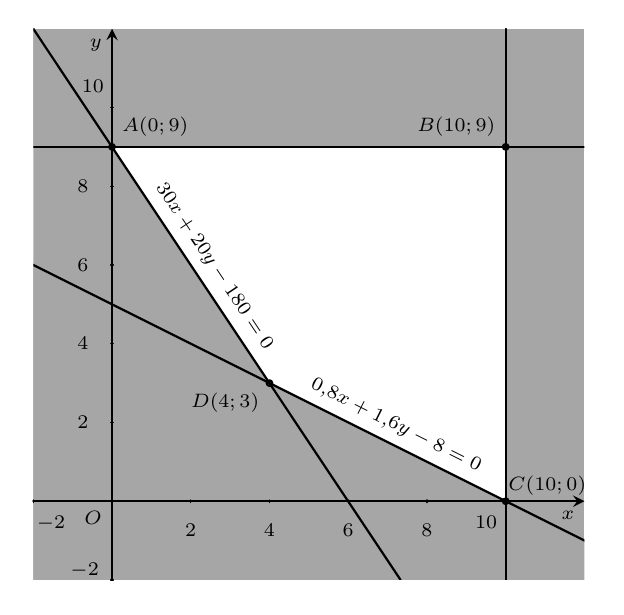
\begin{tikzpicture}[line join=round, line cap=round,>=stealth,thick,scale =.5]
				%	\tikzset{every node/.style={scale=0.9}}
				\begin{scope}
					\clip (-2,-2) rectangle (12,12);
					\fill[black!35] (-3,13.5)--(-3,-10.5)--(13,-10.5)--cycle;
					\fill[black!35] (-15,12.5)--(-15,-2.5)--(15,-2.5)--cycle;
					\fill[black!35] (10,-2)--(12,-2)--(12,12)--(10,12)--cycle;
					\fill[black!35] (-2,9)--(-2,12)--(12,12)--(12,9)--cycle;
					\draw (-2,12)--(7.33,-2)node [pos=0.45, above, sloped,font=\scriptsize] {$30x+20y-180=0$};
					\draw (-14,12)--(14,-2) node [pos=0.75, above, sloped,font=\scriptsize] {$0{,}8x+1{,}6y-8=0$};
					\draw (10,-2)--(10,12);
					\draw (-2,9)--(12,9);
				\end{scope}
				\draw[->] (-2,0)--(12,0) node[below left,font=\scriptsize]{$x$};
				\draw[->] (0,-2)--(0,12) node[below left,font=\scriptsize]{$y$};
				\draw (0,0) node[below left,font=\scriptsize]{$O$};
				\foreach \x/\g in {-2/-50,2/-90,4/-90,6/-90,8/-90,10/225}
				\draw[thin] (\x,1pt)--(\x,-1pt) node [shift={(\g:10pt)},font=\scriptsize] {$\x$};
				\foreach \y/\g in {-2/160,2/180,4/180,6/180,8/180,10/130}
				\draw[thin] (1pt,\y)--(-1pt,\y) node [shift={(\g:10pt)},font=\scriptsize] {$\y$};
				\draw (0,9) circle (2pt) node [above right,font=\scriptsize] {$A(0;9)$};
				\draw (10,9) circle (2pt) node [above left,font=\scriptsize] {$B(10;9)$};
				\draw (10,0) circle (2pt) node [shift={(20:16pt)},font=\scriptsize] {$C(10;0)$};
				\draw (4,3) circle (2pt) node [below left,font=\scriptsize] {$D(4;3)$};
			\end{tikzpicture}	
		\end{center}
		Ta thấy các điểm $A(0;9)$, $B(10;9)$, $C(10;0)$, $D(4;3)$.\\
		Khi này ta có $C_A=36$, $C_B=86$, $C_C=50$, $C_D=32$.\\
		Vậy chi phí thấp nhất là $32$ triệu đồng khi thuê $4$ xe loại $A$ và $3$ xe loại $B$.}
\end{ex}

\Closesolutionfile{ans}
%\inputansbox[2]{2}{ans/0D2.2-KQ}
\begin{center}
	\textbf{Phần 4. Tự luận}
\end{center}
\setcounter{ex}{0}
\begin{bt}%[0D2H2-2]
	Biểu diễn miền nghiệm của hệ bất phương trình
	\begin{itemize}
		\item $\heva{&x+2y<-4\\&y\ge x+5;}$
		\item $\heva{&4x-2y>8\\&x\ge 0\\&y\le 0.}$
	\end{itemize}
	\loigiai{
		\begin{itemize}
			\item 
			\immini{Vẽ các đường thẳng
				\begin{itemize}
					\item $d_1\colon x+2y=-4$; 
					\item $d_2\colon y-x= 5$.
				\end{itemize}
				Gạch đi các phần không thuộc miền nghiệm của mỗi bất phương trình.\\
				Miền nghiệm của hệ bất phương trình là phần không bị gạch bỏ ở hình bên kể cả đường thẳng $d_2$.}
			{
				\begin{tikzpicture}[scale=1, font=\footnotesize, line join=round, line cap=round, >=stealth]
					\begin{scope}[scale=.7]
						\begin{scope}
							\clip (-6,-2.5) rectangle (1,5.5);
							\fill[opacity=.3,pattern=north east lines] (-16,6)--(2,6)--(2,-3)--cycle;
							\fill[opacity=.3,pattern=north west lines] (-8,-3)--(2,-3)--(2,7)--cycle;
							\draw (-15,5.5)--(1,-2.5) node [pos=0.6, above, sloped] {$d_1$};
							\draw (0.5,5.5)--(-7.5,-2.5) node [pos=0.15, above, sloped] {$d_2$};
						\end{scope}
						\draw[->] (-6,0)--(1,0) node[below]{$x$};
						\draw[->] (0,-2.5)--(0,5.5) node[left]{$y$};
						\draw (0,0) node[below left]{$O$};
						\foreach \x in {-5,-4}
						\draw[thin] (\x,1pt)--(\x,-1pt) node [below] {$\x$};
						\foreach \y in {-2,5}
						\draw[thin] (1pt,\y)--(-1pt,\y) node [left] {$\y$};
					\end{scope}
					
				\end{tikzpicture}
			}
			\item 
			\immini{Vẽ các đường thẳng
				\begin{itemize}
					\item $d_1\colon 4x-2y=8$; 
					\item $d_2\colon x= 0$ là trục tung; 
					\item $d_3\colon y= 0$ là trục hoành.
				\end{itemize}
				Gạch đi các phần không thuộc miền nghiệm của mỗi bất phương trình.\\
				Miền nghiệm của hệ bất phương trình là phần không bị gạch bỏ ở hình bên kể cả đường thẳng $d_2$, $d_3$.
			}
			{
				\begin{tikzpicture}[scale=1, font=\footnotesize, line join=round, line cap=round, >=stealth]
					\begin{scope}
						\clip (-1,-4.5) rectangle (2.5,1);
						\fill[opacity=.3,pattern=north east lines] (-2,-8)--(-2,3)--(3.5,3)--cycle;
						\fill[opacity=.3,pattern=north west lines] (0,-4.5)--(-1,-4.5)--(-1,1)--(0,1)--cycle;
						\fill[opacity=.3,pattern=north east lines] (-1,0)--(-1,1)--(2.5,1)--(2.5,0)--cycle;
						\draw (2.5,1)--(-0.25,-4.5) node [pos=0.45, above, sloped] {$4x + -2y + -8=0$};
					\end{scope}
					\draw[->] (-1,0)--(2.5,0) node[below]{$x$};
					\draw[->] (0,-4.5)--(0,1) node[left]{$y$};
					\draw (0,0) node[below left]{$O$};
					\foreach \x in {2}
					\draw[thin] (\x,1pt)--(\x,-1pt) node [below] {$\x$};
					\foreach \y in {-4}
					\draw[thin] (1pt,\y)--(-1pt,\y) node [left] {$\y$};
					
				\end{tikzpicture}
			}
		\end{itemize}
	}
\end{bt}
% Câu 1
\begin{bt}%[0D3V2-6] 
	Mỗi ngày Nga đều dành không quá 30 phút để đọc cả $2$ cuốn sách A, B. Nga đọc được $3$ trang sách A trong $2$ phút, đọc được $2$ trang sách B trong $1$ phút. Gọi $x$, $y$ lần lượt là số phút đọc sách A và số phút đọc sách B. Tìm điều kiện của $x$ và $y$ để Nga đọc được ít nhất $35$ trang sách trong một ngày.
	\loigiai{
		Gọi $x$, $y$ lần lượt là số phút đọc sách A và số phút đọc sách B trong một ngày $(x$, $y > 0)$. Tổng số phút đọc sách không quá $30$ phút nên $x + y \leq 30$.
		
		Số trang sách A đọc được sau $x$ phút là $\dfrac{3x}{2}$. Số trang sách B đọc được sau $y$ phút là $2y$.
		
		Nga đọc được ít nhất $35$ trang sách trong một ngày khi và chỉ khi $\dfrac{3x}{2} + 2y \geq 35$.
		
		Vậy $x$, $y$ cần thỏa mãn các điều kiện
		$
		\heva{
			&x > 0 \\
			&y > 0 \\
			&x + y \leq 30 \\
			&\dfrac{3x}{2} + 2y \geq 35.
		}
		$
	}
\end{bt}
% Câu 2
\begin{bt}%[0D2V2-6] 
	Mỗi ngày Nga đều dành không quá 30 phút để đọc cả $2$ cuốn sách A, B. Nga đọc được $3$ trang sách A trong $2$ phút, đọc được $2$ trang sách B trong $1$ phút. Gọi $x$, $y$ lần lượt là số phút đọc sách A và số phút đọc sách B. Tìm điều kiện của $x$ và $y$ để Nga đọc được ít nhất $35$ trang sách trong một ngày.
	\loigiai{
		Gọi $x$, $y$ lần lượt là số phút đọc sách A và số phút đọc sách B trong một ngày $(x$, $y > 0)$. Tổng số phút đọc sách không quá $30$ phút nên $x + y \leq 30$.
		
		Số trang sách A đọc được sau $x$ phút là $\dfrac{3x}{2}$. Số trang sách B đọc được sau $y$ phút là $2y$.
		
		Nga đọc được ít nhất $35$ trang sách trong một ngày khi và chỉ khi $\dfrac{3x}{2} + 2y \geq 35$.
		
		Vậy $x$, $y$ cần thỏa mãn các điều kiện
		$
		\heva{
			&x > 0 \\
			&y > 0 \\
			&x + y \leq 30 \\
			&\dfrac{3x}{2} + 2y \geq 35.
		}
		$
	}
\end{bt}

%Câu 3
\begin{bt}%[0D2V2-3] 
	Người ta dự định dùng hai loại nguyên liệu $K$, $P$ để sản xuất ít nhất $72$ kg sản phẩm loại $I$ và $80$ kg sản phẩm loại $II$. Từ mỗi tấn nguyên liệu $K$ giá $4$ triệu đồng, có thể sản xuất được $24$ kg sản phẩm loại $I$ và $40$ kg sản phẩm loại $II$. Từ mỗi tấn nguyên liệu $P$ giá $3$ triệu đồng, có thể sản xuất được $36$ kg sản phẩm loại $I$ và $20$ kg sản phẩm loại $II$. Hỏi phải dùng bao nhiêu tấn nguyên liệu mỗi loại để chi phí mua nguyên liệu là ít nhất? Biết rằng cơ sở cung cấp nguyên liệu chỉ có thể cung cấp tối đa $3$ tấn nguyên liệu loại $K$ và $4$ tấn nguyên liệu loại $P$.
	\loigiai{
		Gọi $x$, $y$ (tấn) lần lượt là số tấn nguyên liệu loại $K$ và $P$ cần mua. Khi đó $x \ge 0$, $y \ge 0$.\\
		Chi phí để mua $x$ tấn nguyên liệu $K$ và $y$ tấn nguyên liệu $P$ là $F(x;y)=4x+3y$ (triệu  đồng).\\
		Vì cơ sở cung cấp nguyên liệu chỉ có thể cung cấp tối đa $3$ tấn nguyên liệu loại $K$ và $4$ tấn nguyên liệu loại $P$ nên $x \le 3$, $y \le 4$.\\
		Vì cần sản xuất ít nhất $72$ kg sản phẩm loại $I$ và $80$ kg sản phẩm loại $II$ nên $24x+36y \ge 72$, $40x+20y \ge 80$.\\
		Từ đó ta thu được hệ bất phương trình sau:
		$$\heva{&0\le x \le 3\\&0\le y \le 4\\&24x+36y \ge 72\\&40x+20y \ge 80} \Leftrightarrow \heva{&0\le x \le 3\\&0\le y \le 4\\&2x+3y \ge 6\\&2x+y \ge 4.}$$
		Biêu diễn miền nghiệm của hệ bất phương trình trên mặt phẳng tọa độ, miền nghiệm là phần trong của tứ giác $ABCD$ (kể cả các cạnh của tứ giác) với $A(0;4)$, $B(3;4)$, $C(3;0)$ và $D(1;1{,}5)$.
		\begin{center}
			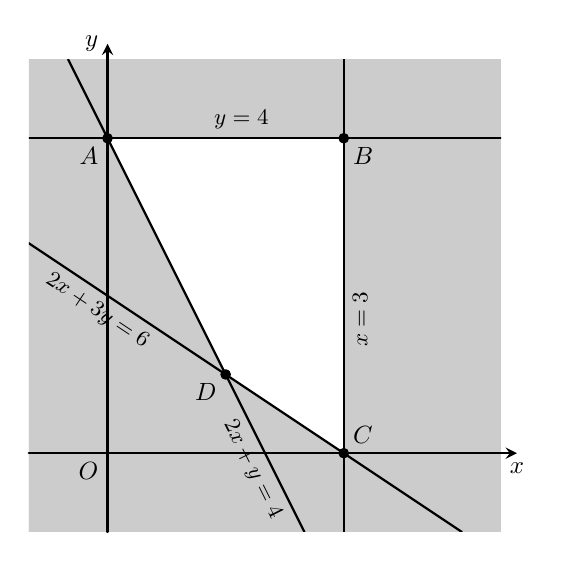
\begin{tikzpicture}[line join=round, line cap=round,>=stealth,thick]
				\tikzset{every node/.style={scale=0.9}}
				\begin{scope}
					\clip (-1,-1) rectangle (5,5);
					\fill[gray!40] (-5,5.33)--(-5,-2)--(6,-2)--cycle;
					\fill[gray!40] (-2,8)--(-2,-8)--(6,-8)--cycle;
					\fill[gray!40] (3,-1)--(5,-1)--(5,5)--(3,5)--cycle;
					\fill[gray!40] (-1,4)--(-1,5)--(5,5)--(5,4)--cycle;
					\fill[gray!40] (0,-1)--(-1,-1)--(-1,5)--(0,5)--cycle;
					\fill[gray!40] (-1,0)--(-1,-1)--(5,-1)--(5,0)--cycle;
					\draw (-4.5,5)--(4.5,-1) node [pos=0.5, below, sloped] {\small $2x+3y=6$};
					\draw (-0.5,5)--(2.5,-1) node [pos=0.85, below, sloped] {\small $2x+y=4$};
					\draw (3,-1)--(3,5) node [pos=0.45, below, sloped] {\small $x=3$};
					\draw (-1,4)--(5,4) node [pos=0.45, above, sloped] {\small $y=4$};
				\end{scope}
				\draw[->] (-1,0)--(5.2,0) node[below]{$x$};
				\draw[->] (0,-1)--(0,5.2) node[left]{$y$};
				\draw (0,0) node[below left]{$O$};
				\draw[fill=black] (0,4)circle(1.5pt) node[below left]{$A$}
				(3,4)circle(1.5pt) node[below right]{$B$}
				(3,0)circle(1.5pt) node[above right]{$C$}
				(1.5,1)circle(1.5pt) node[below left]{$D$}
				;
			\end{tikzpicture}
		\end{center}
		Ta có $F(0;4)=12$, $F(3;4)=24$, $F(3;0)=12$ và $F(1;1{,}5)=8{,}5$. Nên giá trị nhỏ nhất cần tìm là $F(1;1{,}5)=8{,}5$.\\
		Vậy dùng $1$ tấn nguyên liệu loại $K$ và $1{,}5$ tấn nguyên liệu loại $P$ thì chi phí mua nguyên liệu là ít nhất.
	}
\end{bt}






